\documentclass[12pt,a4paper]{article}
\synctex=1
\usepackage[utf8]{inputenc}
\usepackage[margin=1cm]{geometry}
\usepackage{graphicx}
%\usepackage{verbatim}
\usepackage{amsmath}
\usepackage{amsfonts}
\usepackage{amssymb}
\usepackage{listings}
\usepackage{enumitem}
\usepackage{textcomp}
\usepackage{courier}
\usepackage{libertine}
\usepackage{pgfornament}
\usepackage{eso-pic}
\usepackage[hangul]{kotex}
\linespread{1.3}

\title{
	\centering
	\pgfornament[width=12cm,color=teal]{84}\\
	\vspace{1cm}
	\fontsize{50}{50} \selectfont {정보통신 수학 및 실습\\Homework}\\
		\pgfornament[width=12cm,color=teal]{88}\\
	\vfill}
\author{
	\LARGE
	\begin{tabular}{rl}
		\hline
		학번 : & 2016110056\\ 
		학과 : & 불교학부 \\
		이름 : & 박승원\\
		날짜 : & \today\\
		\hline
	\end{tabular}\vspace{2cm}
	\\
\includegraphics[width=0.5\textwidth]{logo.jpg}
	}
\date{}


\begin{document}
\maketitle
\pagenumbering{gobble}
\noindent
\lstset{language=matlab, columns=flexible, tabsize=4, frame=shadowbox, showstringspaces=false, breaklines=true, upquote=true, basicstyle=\normalsize}

\renewcommand{\thesubsubsection}{\alph{subsubsection})}
\renewcommand{\thesubsection}{\arabic{subsection}.}
\newpage

\section*{Chapter 6 Homework}
Show your solutions and do not use MATLAB for your homework except Problem 5.

\subsection{Let A=[1 2 3;4 5 6], B=[1 -1;0 1], C=[-1 0;1 1;0 1], D=[-3 -2 -1;1 2 3].  Compute the followings:} 

\subsubsection{$A – C^T$} 
$\begin{bmatrix}
	2&1&3\\
	4&4&5
\end{bmatrix}
$
\subsubsection{$C^T +3D$} 
$
\begin{bmatrix}
-10 &-5& -3\\3& 7& 10
\end{bmatrix}
$
\subsubsection{BA}
$
\begin{bmatrix}
-3&-3&-3\\4&5&6
\end{bmatrix}
$
\subsubsection{CB}
$
\begin{bmatrix}
-1&1\\1&0\\0&1
\end{bmatrix}
$
\subsubsection{$B^3$}
$
\begin{bmatrix}
1 &-3\\0&1
\end{bmatrix}
$
\subsection{For each of the given matrices, find the inverse or determine that the matrix is singular.}

\subsubsection{[1 -1; -1 1]} 
ad - bc = 0이므로 singular
\subsubsection{[1 2;3 4]}
$
\begin{bmatrix}
	-2 &1\\ \dfrac{3}{2} & \dfrac{1}{2}
\end{bmatrix}
$
\subsubsection{[1 2 3;4 5 6; 7 8 9]}
\begin{gather*}
\begin{bmatrix}
	1&2&3\\4&5&6\\7&8&9
\end{bmatrix}\\
A^{-1} = \dfrac{adj(A)}{det(A)}\\
det(A) = \displaystyle\sum_{i=1}^{n}a_{ij}C_{ij}=a_{11}C_{11}+a_{21}C_{21}+a_{31}C_{31}\\
C_{ij} = (-1)^{i+j}M_{ij}\\
det(A)=1\times (45-48) - 4\times (18-24) + 7\times (12-15) = -3 + 24 -21 = 0\\
\therefore singular
\end{gather*}
\subsubsection{[1 2 3; 1 3 2;0 1 1]}
\begin{gather*}
\begin{bmatrix}
1&2&3\\1&3&2\\0&1&1
\end{bmatrix}\\
det(A) = 1\times 1 - 1\times -1 + 0 = 2\\
adj(A) = 
\begin{bmatrix}
C_{11}&C_{12}&C_{13}\\C_{21}&C_{22}&C_{23}\\C_{31}&C_{32}&C_{33}
\end{bmatrix}^T=
\begin{bmatrix}
1&-1&1\\1&1&-1\\-5&1&1
\end{bmatrix}^T=
\begin{bmatrix}
1&1&-5\\-1&1&1\\1&-1&1
\end{bmatrix}
\\
A^{-1}=\dfrac{adj(A)}{2}=
\begin{bmatrix}
0.5& 0.5&-2.5\\-0.5&0.5&0.5\\0.5&-0.5&0.5
\end{bmatrix}\\
\end{gather*}
\subsection{Write each of the following linear equation as a matrix equation, and solve by inverting the coefficient matrix} 
\begin{gather*}
x + y + z = 2\\
x +2y + z = 6\\
y + z = 1\\
\begin{bmatrix}
1&1&1\\1&2&1\\0&1&1
\end{bmatrix}
\begin{bmatrix}
x\\y\\z
\end{bmatrix}
=
\begin{bmatrix}
2\\6\\1
\end{bmatrix}\\
det(A) = 1\\
adj(A) = 
\begin{bmatrix}
1&-1&1\\0&1&-1\\-1&0&1
\end{bmatrix}^T=
\begin{bmatrix}
1&0&-1\\-1&1&0\\1&-1&1
\end{bmatrix}\\
\therefore A^{-1} = 
\begin{bmatrix}
1&0&-1\\-1&1&0\\1&-1&1
\end{bmatrix}\\
\begin{bmatrix}
x\\y\\z
\end{bmatrix}
=
\begin{bmatrix}
1&0&-1\\-1&1&0\\1&-1&1
\end{bmatrix}
\begin{bmatrix}
2\\6\\1
\end{bmatrix}
=
\begin{bmatrix}
1\\4\\-3
\end{bmatrix}
\end{gather*}



\subsection{Find a matrix A which rotates a point by 60 degree clockwise .  Draw Ax when x is on a unit square as follows:\\(1.1)}

\begin{gather*}
\begin{bmatrix}
	\cos(-60)& -\sin(-60)\\ \sin(-60)& cos(-60)
\end{bmatrix}
=
\begin{bmatrix}
0.5&\dfrac{\sqrt{3}}{2}\\-\dfrac{\sqrt{3}}{2}&0.5
\end{bmatrix}\\
\begin{bmatrix}
0.5&\dfrac{\sqrt{3}}{2}\\-\dfrac{\sqrt{3}}{2}&0.5
\end{bmatrix}
\begin{bmatrix}
0&1&0&1\\0&0&1&1
\end{bmatrix}
=
\begin{bmatrix}
0&0.5&\dfrac{\sqrt{3}}{2}&\dfrac{1+\sqrt{3}}{2}\\
0&-\dfrac{\sqrt{3}}{2}&0.5&\dfrac{1-\sqrt{3}}{2}
\end{bmatrix}
\end{gather*}
\begin{center}
	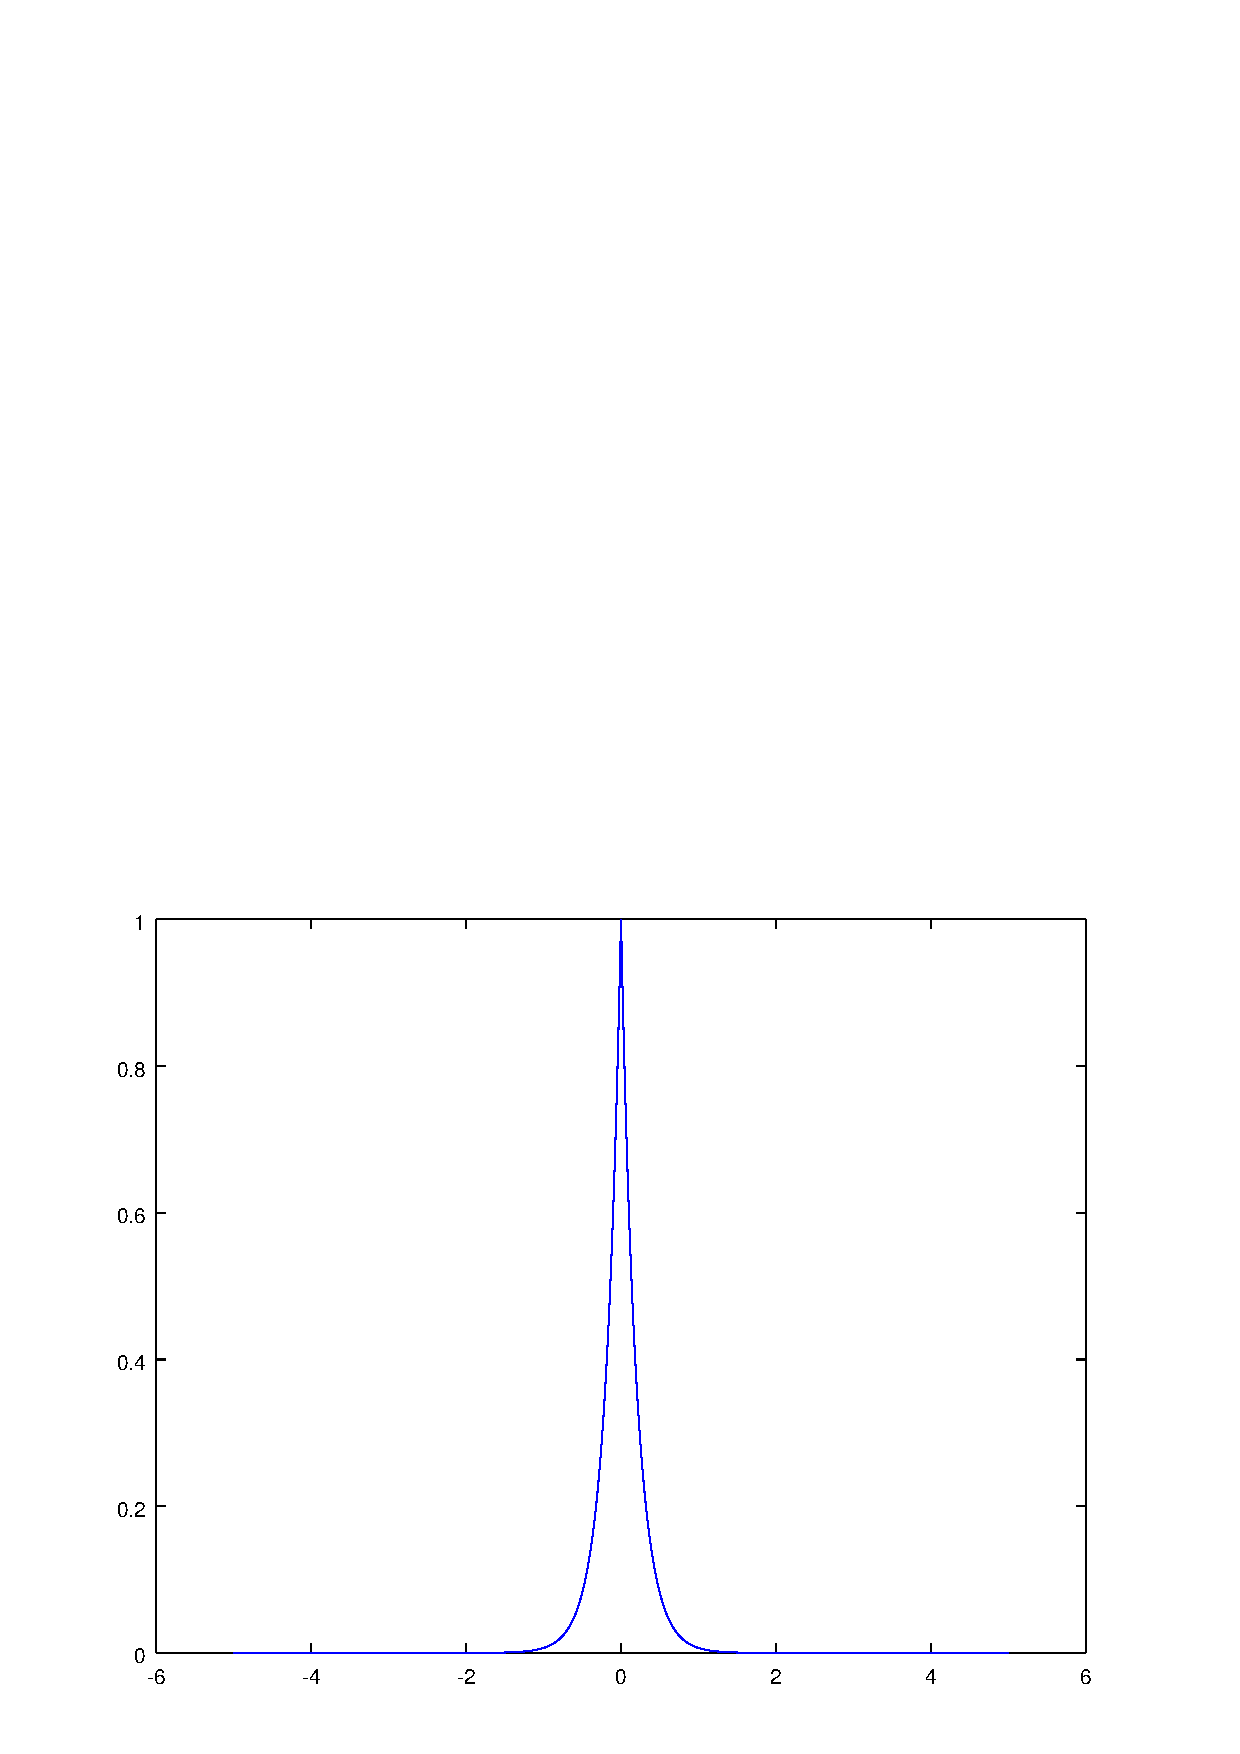
\includegraphics[width=0.8\textwidth]{2.png}
\end{center}

\subsection{Find the Eigen values and Eigen vectors of A = [9 14; 1 4] and draw the trace of Ax if x is a vector on the unit circle using MATLAB.  Then calculate $A^5$ using MATLAB. } 

\begin{gather*}
Av = \lambda v\\
det(A-\lambda I) = 0\\
\end{gather*}

\begin{equation*}
	\begin{Vmatrix}
	9-\lambda&14\\1&4-\lambda
	\end{Vmatrix}=0\\
\end{equation*}
	
\begin{gather*}
36 -13\lambda + \lambda^2 -14 = 0\\
(\lambda-11)(\lambda-2)=0\\
\rhd \lambda=11\\
\begin{bmatrix}
-2&14\\1&-7
\end{bmatrix}
\begin{bmatrix}
x\\y
\end{bmatrix}=0\\
v = k
\begin{bmatrix}
1 \\-7
\end{bmatrix}\\
\rhd \lambda=2\\
v=k
\begin{bmatrix}
1\\2
\end{bmatrix}\\
\end{gather*}
\begin{lstlisting}
th = linspace(0, 2*pi, 100);
x = cos(th);
y = sin(th);
A = [9 14; 1 4]
B = A * [x;y];
t = linspace(-0.5,0.5,100);
plot(x,y, B(1,:), B(2,:), t, -7*t, t, 2*t)
\end{lstlisting}

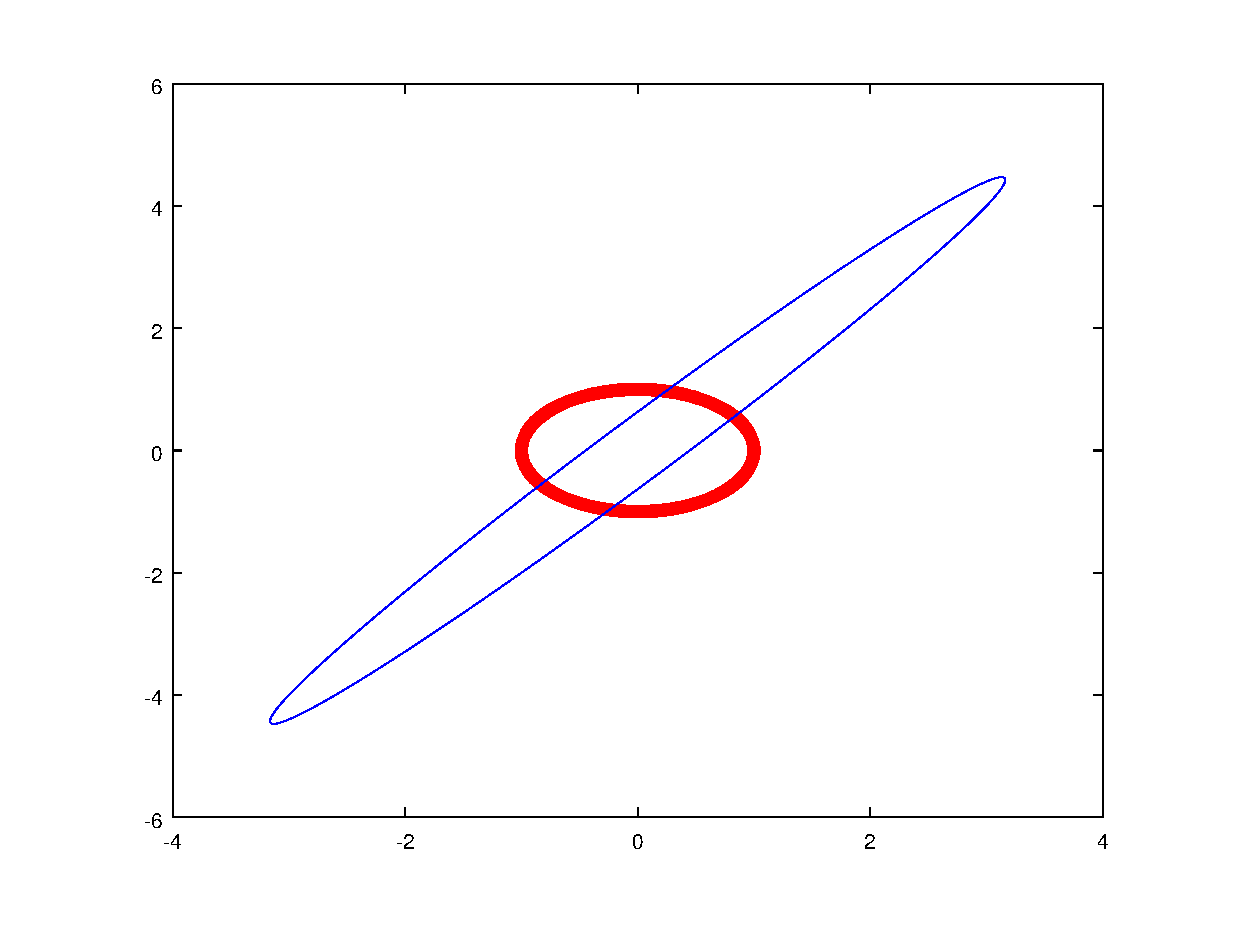
\includegraphics[width=0.8\textwidth]{5.eps}
\begin{gather*}
\text{\Large Matrix decomposition}\\
V = [v_1, v_2]=
\begin{bmatrix}
1&1\\-7&2
\end{bmatrix}\\
AV = 
\begin{bmatrix}
9&14\\1&4
\end{bmatrix}
\begin{bmatrix}
1&1\\-7&2
\end{bmatrix}=\lambda V = 
[11v_1, 2v_2]=
\begin{bmatrix}
1&1\\-7&2
\end{bmatrix}
\begin{bmatrix}
11&0\\0&2
\end{bmatrix}
=V\Lambda\\
\therefore A^5=M\Lambda^5M^{-1}=
\begin{bmatrix}
1&1\\-7&2
\end{bmatrix}
\begin{bmatrix}
11^5&0\\0&2^5
\end{bmatrix}
\dfrac{1}{9}
\begin{bmatrix}
2&-1\\7&1
\end{bmatrix}=
\begin{bmatrix}
 125269 &  250474\\
 17891   & 35814
\end{bmatrix}
\end{gather*}


\end{document}
